\documentclass[12 pt]{article}
\usepackage{fullpage}
\usepackage{amsthm}
\usepackage{amsmath}
\usepackage{xcolor}
\usepackage{amssymb}
\usepackage{graphicx}
\usepackage{hyperref}
\usepackage{setspace}

\doublespacing

\hypersetup{colorlinks=true, linkcolor=blue}

\newcommand{\new}[1]{\bigskip \noindent \color{blue} \textbf{#1}\medskip}
\newcommand{\q}[1]{\response{\emph{#1}}}
\newcommand{\prompt}[1]{\noindent \textbf{#1}}
\newcommand{\response}[1]{\color{black} #1 \medskip}
\newcommand{\bb}[1]{\mathbb{#1}}
\newcommand{\pset}[1]{\mathcal{P}({#1})}

\newcommand{\Q}[2]{\new{Question {#1}:} \q{#2}}
\newcommand{\proposition}[1]{\prompt{Proposition:} \response{#1}}
\newcommand{\discussion}[2]{\\ \prompt{Discussion:} \begin{itemize}
    \item \prompt{What we know:} {#1}
    \item \prompt{What we'll do:} {#2}
\end{itemize}}
\newcommand{\p}[1]{\begin{proof} \response{{#1}} \end{proof}}
\newcommand{\con}[1]{\\ \prompt{Conjecture:}\response{#1}}

\begin{document}

\topskip0pt
\begin{center} \normalsize California Institute of Technology \\ \end{center}
\vspace*{\fill}
\begin{center}
    \Large When to Pull a Pitcher? Predicting Drops in Pitcher Effectiveness in 
    Major League Baseball \color{black}
\end{center}
\vspace*{\fill}
\begin{center} \normalsize Edward Speer\\ \end{center}
\begin{center} \normalsize BEM/Ec 120: Sports Science\\ \end{center}
\begin{center} \normalsize Dr. R. Micheal Alvarez and Dr. Oliver Eslinger\\ \end{center}
\begin{center} \normalsize May 17, 2023\\ \end{center}


\pagebreak

\textbf{I. Introduction} \\

\indent In baseball, one of the most critical and notoriously difficult strategic 
decisions to make is when to remove one pitcher from the game and put another in.
This decision is based on a wide range of game features, including hitter-pitcher 
matchups, game importance, bullpen rest, and many other factors. However, the most 
crtical factor, and yet the most difficult to judge, is pitcher fatigue. As a pitcher 
becomes either physically or mentally tired, they naturally become less effective
in preventing the other team from scoring. However, pitcher fatigue can manifest itself in ways 
that vary between pitchers, and often may only clearly show itself after the opposing 
team has already gained an offensive advantage. The goal of this paper is to propose 
a sabermetrics approach which uses sliding in game pitch metrics to determine when a 
pitcher is growing fatigued, before enabling the other team to take advantage.
\\ \indent In baseball, throughout most games the personnel in the game remain largely te same. 
Starters typically play a whole game, without the frequent substitutions expected 
in other sports. The major exception to this is the pitcher, who is expected to be substituted 3 or 4
times throughout the game. The pitcher also has the largest effect on a team's 
defense by virtue of their role. This makes the substitution of the pitcher 
a very weighty decision in the game with large ramifications, and consequently one of 
the decisions of a baseball manager underrth largest scrutiny. The game importance and 
visibility of these decisions make it important to develop metric based methods which 
optimize their result. 
\\ \indent Baseball pitchers are highly varied athletes. The MLB recognizes 13 
different types of pitches, with each pitcher in the league throwing a
different combination of pitches (called their pitch arsenal), each of which has 
unique characteristics when thrown by one arm over another. This incredible variety 
in pitchers makes it difficult to generalize any conclusions from sabermetrics 
across pitchers. This paper's approach is to use data clustering techniques to 
sort pitchers into distinct archetypes based on their pitch arsenals, and then 
look at specific indicators from game data to uncover indicators of pitcher fatigue 
common to each pitcher cluster. This allows for an additional measure of specificity 
allowing the result to apply generally enough for ease of use across MLB pitchers, 
but enough specificity to be insightful.
\\ \indent Recognizing the characteristic fatigue signals of different archetypes of 
pitchers in the MLB is widely applicable beyond the limits of MLB pitchers. In youth and 
amateur sports, many pitchers pattern themselves after professional pitchers, throwing similar 
arsenals, or arsenals which can be sorted into the same archetypes as MLB pitchers. 
Recognizing the pitcher archetype in combination with fatigue markers for their pitchers can allow 
managers at all levels of baseball to make informed decisions about when to change pitchers, 
even with decreased access to advanced game data. \\

\textbf{II. Review of Literature} \\ \\ 
\indent Research into pitcher removal from a game has been somewhat sparse, and has 
focused mainly on how managers currently make decisions as opposed to how optimal 
decision making could be performed. These studies have attempted to determine or measure 
managers act as they do, and if their decision making is optimal, and have revealed the
need for this study by showing sub-optimal behavior in this decision making. Phillips' 2017 
study showed that managers emphasize pitch count disproportionately when removing pitchers, 
showing a strong tendency to remove pitchers on pitch counts which are multiples of 
10 regardless of the game state, with no clear statistical reason for this behavior [1]. 
Clearly this shows managerial behavior which is subjective and not driven by sabermetrics. 
\\ \indent Grantham et al. looked at college pitchers, and showed that pitcher fatigue 
significantly impacted pitching mechanics over the course of a game, with pitchers showing 
clear biophysical indicators of fatigue with increased number of pitches or innings thrown[2]. 
For the purposes of this paper, we hypothesize that these biophysical differences in pitching mechanics
will result in observable changes in the metrics surrounding ball flight. For example, Grantham found that external rotation 
was strongly impacted by pitcher fatigue. A decrease in external rotation likely results in 
decreased pitch velocity, which is observable from the sabermetrics used in this paper.
\\ \indent Whiteside et al. 2016 found that the variables which changed the most 
over the course of a pitchers performance as the pitcher fatigued were pitch 
velocity, vertical movement, and proportion of offspeed pitches thrown by the pitcher. However, 
these variables were not strongly correlated with effectiveness [3]. This paper seeks to find markers 
hidden in these and other pitching metrics which both change as a pitcher fatigues and 
have a stronger correlation with effectiveness than those found by Whiteside.
\\ \indent Woodham et al. 2019 used a machine learning model to identify the most 
significant features in when a starting pitcher would be removed from a game in an effort 
to predict when a starting pitcher should be removed, and found that the strike count 
and number of batters a pitcher has faced in the game, in conjunction with the number of outs, 
inning number, and number of homeruns allowed are the most significant factors in removing a pitcher [4]. 
However, these conclusions yield sparse information in how to make decisions about removing a pitcher, 
as they are very standard metrics of performance, and if a pitcher is performing poorly 
(throwing balls and giving up homeruns), then it is evident they must be removed 
from the game. An improved predictive model would anticipate from markers in the sabermetric 
data when the pitcher was going to give up homeruns or walks, and remove the pitcher prior to allowing 
that advantage to the offensive team.
\\ \indent Each of these previous studies show that pitcher fatigue is observable in 
in-game metrics seen throughout the course of the game. Combining this observation with a 
study of the in-game pitching metrics available from the modern MLB statcast system should 
allow the development of a predictive model which correlates markers of pitcher fatigue with 
oncoming increases in offensive output by an opposing team. \\

\textbf{III. Theory and Hypothesis} \\ \\
\indent Due to the wide variability in pitcher mechanics and style across pitchers in the 
MLB, it is clear that different pitch metrics will impact the effectiveness of 
pitchers in different ways. For example, a pitcher who throws a changeup 10\% of the time will likely 
be far less effected in their ability to get outs by a reduction in their changeup metrics than 
a pitcher who throws a changeup 50\% of the time. As a result, the first step to developing 
a predictive model of which variables impact pitching performance is to sort 
pitchers into categories, with pitchers in each category of pitcher being likely to 
to have their effectiveness impacted by the same metrics. This way the predictions of 
the model can still be generalized across a larger group of pitchers while still having a measure of 
precision. This means there will be some inherent trade-off between the granularity of the 
pitcher grouping and the accuracy of the predictions which will need to be fine-tuned 
for the desired results.
\\ \indent A pitcher's arsenal is the set of pitches that a pitcher uses combined 
with the frequency and characteristics with which they throw each pitch. The characteristics 
of a pitch are metrics like the speed, spin rate, and spin axis that characterize the flight 
and shape of the pitch. A pitcher's arsenal combined with their longevity, handedness, and the opponent 
completely determine the strategy of how a pitcher will be used.
\\ \indent The best way to cluster pitchers will be based on their pitch arsenal. 
Pitching style is captured the best by how hard pitchers throw, which different pitches 
they throw, and how often they throw different pitches. Other factors which might tend 
to be included in a clustering are pitcher handedness and pitcher arm angle, however 
these factors are unlikely to be impacted by fatigue and therefore may be excluded from 
a clustering intended to reveal fatigue characteristics.
\\ \indent With this clustering of pitchers grouping similar arsenals together, 
an analysis of common fatigue characteristics may then be carried out. Grantham et al. showed 
that fatigue changes the mechanics of a pitcher's delivery over the course of a game, and 
with changes in mechanics come changes in the characteristics of the flight of the 
ball out of the pitcher's hand. Any subtle change in the pitcher's arm angle will cause 
a change in the spin axis of the ball. Muscle fatigue will show a change in pitch velocity, 
and forearm musce fatigue will show a reduction in spin rate. Any of these factors can be observed 
from in-game statcast data. 
\\ \indent Notably absent from this discussion of when to remove a pitcher is
the current opponent and opposing batter. These factors clearly will influence the 
optimal time to remove a pitcher, since pitchers match up more or less favorably against 
certain opponents. However, the goal of this study is to determine how markers of pitcher 
fatigue can be observed to understand the current effectiveness of the pitcher, and 
a manager could consider these markers in conjunction with the opponent to inform 
pitching decisions. For instance if a pitcher belonged to a cluster with curve ball spin 
rate identified as a predictor of effectiveness, and the manager observed a sliding 
reduction in the pitcher's spin rate and knew that the upcoming hitter has historically 
performed will in this matchup, then the manager could use the spin rate in order to 
inform his decision to remove the pitcher. Performing the analysis in this opponent-agnostic 
way allows the development of simpler predictions which may be applied more widely. In the 
future similar analysis could be carried out to analyze certain matchups, however this 
study is more concerned with identifying more general pitcher fatigue tendencies that 
impact their performance.
\\ \indent It is hypothesized that for each cluster identified in the paper, the combination 
of variables which is most important for each pitcher to remain effective throughout a game 
are the speed of the primary pitch, combined with either the spin axis or spin rate of the 
secondary pitch. This group of variables indicates a pitcher's ability to throw 
a primary pitch at a speed which is competitive, and a secondary pitch with good movement, 
a combination of features which is traditionally sought after in baseball. However, it is 
suspected that some clusters will deviate from this behavior, as some clusters will likely not 
throw any pitches at a high speed, in which case primary pitch speed shouldn't 
provide as much of an indicator of pitcher effectiveness. However, it is likely that 
for these clusters as well the best indicators of fatigue contributing to a breakdown 
in effectiveness will be some combination of features of primary and secondary pitches, as it 
is typically the combination of multiple pitches which make an arsenal effective. \\

\textbf{IV. Data and Methods} \\ \\
\indent In order to select data to use for this study, it was important to consider 
several confounding factors which could alter the consistency of pitching data. 
Firstly, pitcher tendencies change from year to year, with pitchers adding or removing 
pitches from their arsenals and changing the characteristics of the pitches in their 
arsenals in the offseason. Sometimes, this change could even be drastic enough to change the 
cluster which a pitcher could belong to in a clustering analysis. Therefore, clearly, 
data must be selected from a single season. The most recent available full season is 2022 data, however
halfway through the 2022 season, the MLB implemented new substance control policies 
relating to pitchers which caused sharp changes in the spin rates of different pitchers 
across the league, making the data too inconsistent for this analysis. Therefore the 2021 season was selected.
\\ \indent Baseball Savant is a website owned and operated by the MLB which makes 
publically available advanced metrics taken from MLB games Their data set of pitching 
metrics from 2017 is extensive and contains all the data used for any of the analysis which 
follows. 
\\ \indent In order to cluster MLB pitchers into distinct archetypes, the following 
statistics are scraped for all pitchers who threw a minimum of 1000 pitches in 2021:
\begin{center}
    \begin{tabular}{||c | l||} 
     \hline
     Metric & Description  \\ [0.5ex] 
     \hline
     Average Speed & The speed of a pitch in miles per hour, averaged over all the
     pitches of that \\ & type thrown by the pitcher. \\
     \hline
     Average Spin & The rate at which a pitch spins, measured in rotations per minute, \\
     & averaged over all the pitches of that type thrown by the pitcher. \\
     \hline
     Use Percentage & The percent of pitches thrown by the pitcher which are this type of pitch. \\
     \hline
    \end{tabular}
    \newline \\ Table 1: Pitching Arsenal Metrics
\end{center}
\indent Each of these metrics are scraped for each type of pitch thrown by each pitcher, 
providing a characterization for each pitcher of what pitches they throw, with what speed 
and movement (for full data see appendix I). The pitches thrown in 2021 include the 
following pitch types: 

\begin{center}
    \begin{tabular}{||c | c | l||} 
     \hline
     Pitch & Data Label & Description  \\ [0.5ex] 
     \hline
     4-Seamer & ff & A fast, straight fastball with close to vertical backspin \\
     \hline
     Sinker & si & A fastball that drops vertically over the course of its flight \\
     \hline
     Cutter & fc & A fastball which curves horizontally toward the glove side of the\\
     && pitcher\\
     \hline
     Slider & sl & A "breaking ball" (pitch with an arcing path) which moves mostly 
     \\ && horizontally toward the pitcher's glove side\\
     \hline
     Changeup & ch & A slower pitch whose flight is straight with some dropping vertical\\ 
     && Movement.\\
     \hline 
     Curve & cu & A breaking ball whose movement is primarily vertical, dropping\\
     && sharply over the course of its flight \\
     \hline 
     Splitter & fs & A slower pitch with lower spin rate that drops as it approaches home \\
     && plate.\\
     \hline
     Sweeper & st & A breaking ball which breaks exactly horizontal in its flight path \\
     \hline 
     Slurve & sv & A breaking ball which breaks at a 45 degree angle between horizontal 
     \\ && and vertical movement \\
     \hline
    \end{tabular}
    \newline \\ Table 2: Pitch Types
\end{center}

\indent K-means clustering is used to identify clusters of pitchers representing 
distinct pitching styles based on the arsenals thrown by each pitcher. The input 
vectors are the sets of arsenal data for each pitcher, pre-processed by applying mean normalization and 
dividing by the standard deviation of each feature across the entire population. For those 
features which are not populated (i.e a pitcher who does not throw a certain pitch), the absence of the 
feature is actually a key feature of the dataset, as they pitcher not throwing that pitch certainly says something about their strategy.
Therefore in order to capture this information in the data, we assume that features are approximately normally distributed 
across pitchers, and define empty features as a significant deviation from the mean, initializing all values of the
mean normalized empty feature to 4 standard deviations from the mean.
 \\ \indent In order to identify the number of clusters which should be distinguished by k-means, the 
elbow method is used in which clusterings of different sizes are applied until 
an approximate convergence of clustering inertia, defined as the reduction of mean distance from the centroid of each cluster, 
is reached, shown for the pitching arsenal data in the following plot:\\

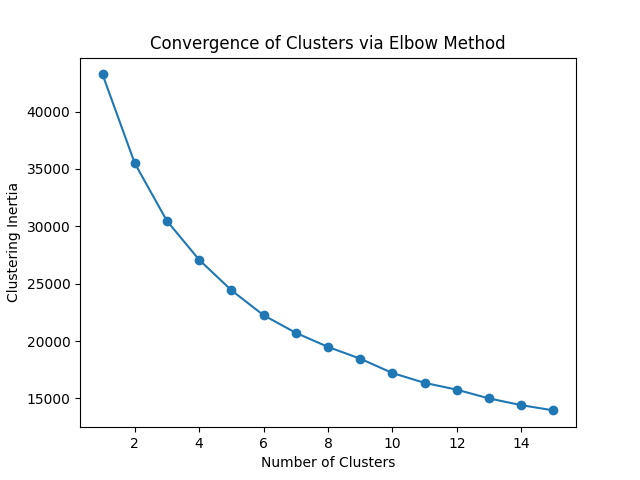
\includegraphics{figs/cls_iner.png}
\begin{center}Figure 1: K-means Clustering Elbow Method\end{center}

\indent In order to minimize clustering inertia while maximizing the amount of information conveyed through 
clustering, a clustering size of 8 is selected and pitchers are sorted accoring to this 
clustering. The results of the clustering are 8 groups of pitchers with distinct 
styles of pitching, characterized best by the frequency with which they throw different pitches. 
These frequencies are shown in the plots below in standard deviations from the average pitch usage, with any 
blank bars indicating that the cluster of pitchers does not throw that pitch.
\begin{center}
 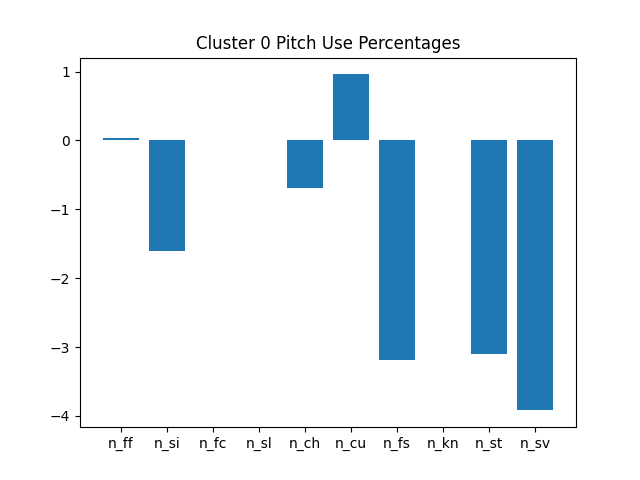
\includegraphics[scale=.425]{figs/pct0_8.png} 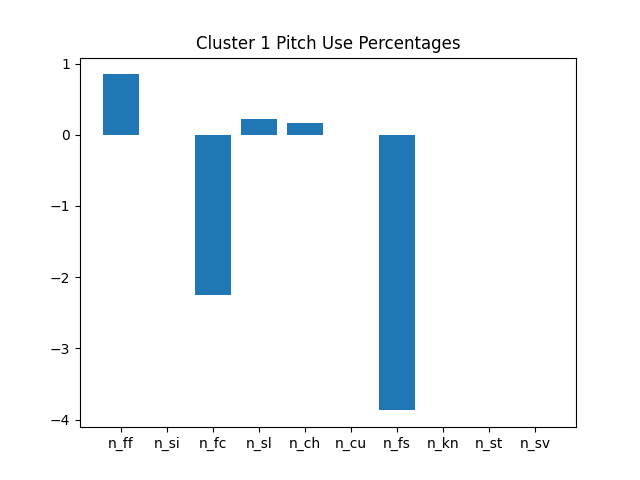
\includegraphics[scale=.425]{figs/pct1_8.png}
\\ 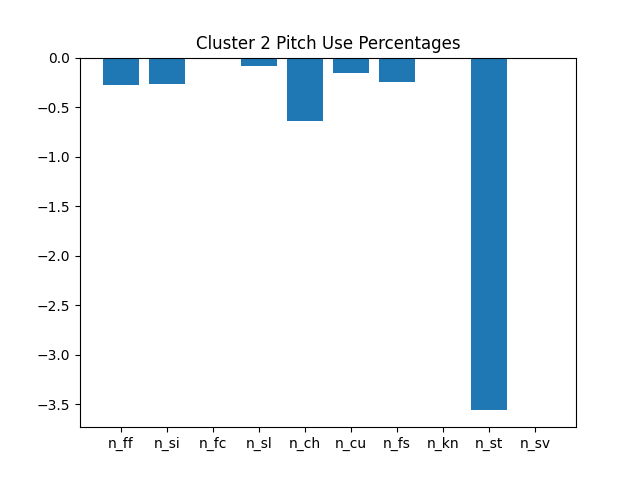
\includegraphics[scale=.425]{figs/pct2_8.png} 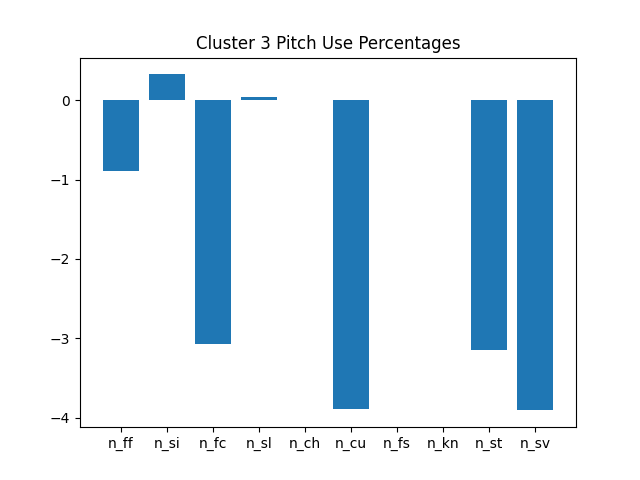
\includegraphics[scale=.425]{figs/pct3_8.png}
\\ 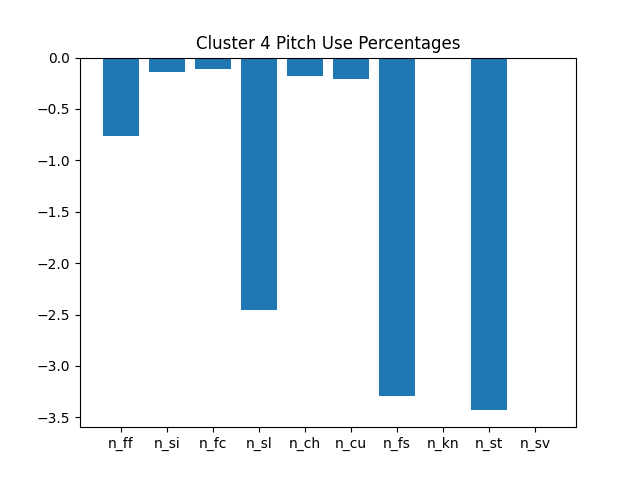
\includegraphics[scale=.425]{figs/pct4_8.png} 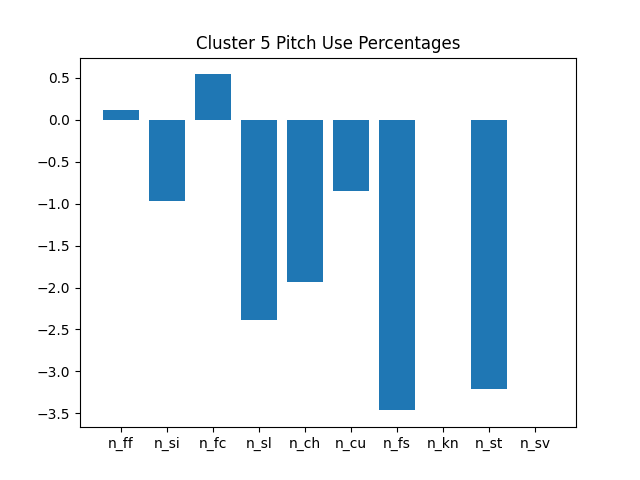
\includegraphics[scale=.425]{figs/pct5_8.png}
\\ 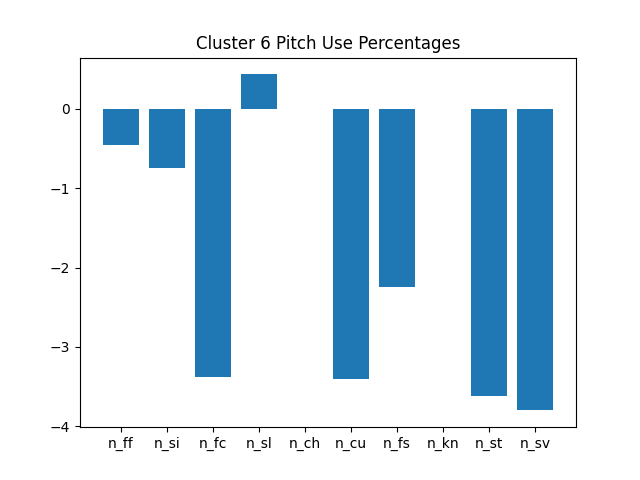
\includegraphics[scale=.425]{figs/pct6_8.png} 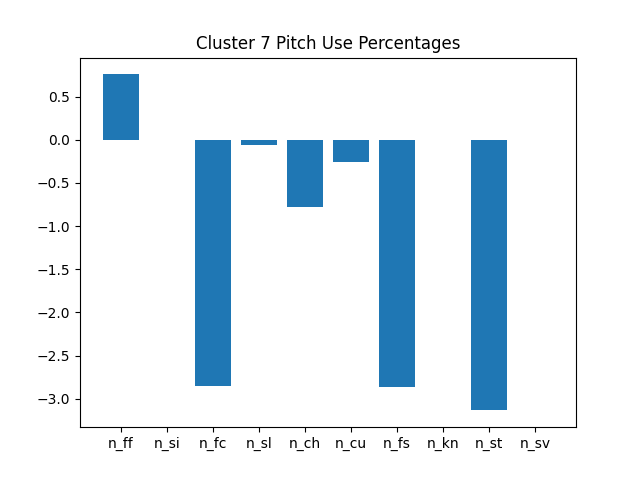
\includegraphics[scale=.425]{figs/pct7_8.png}
\\ Figures 2-9: Cluster Pitch Usages
\end{center}

\indent A clear characterization of each cluster can be observed from these plots of 
pitch usage: 

\begin{center}
    \begin{tabular}{||c | l||} 
     \hline
     Cluster & Description  \\ [0.5ex] 
     \hline
     0 & Changeup heavy pitchers. These pitchers throw a combination of fastball and\\
     & changeup, heavily favoring the changeup as their best pitch, and using their\\
     & fastball as a change in speed to increase the effectiveness of their changeup.\\
     \hline 
     1 & Power fastball pitchers. These pitchers throw far more fastballs than the rest\\
     & of the league, using their fastball in combination with occassional breaking balls\\
     & to get outs.\\
     \hline
     2 & 2-seam pitchers. These pitchers put a lot of movement on their fastballs, both\\
     & cutting them and sinking them, without and blending them with the occassional\\ 
     & straight fastball and changeup, but without relying too heavily on any one pitch.\\
     \hline 
     3 & Sinker ball pitchers. Rely heavily on the sinker to get outs, and mix it with\\
     & the occassional slider.\\
     \hline 
     4 & Nothing straight. These pitchers throw far less straight fastballs than other\\ 
     & clusters of pitchers, relying on moving fastballs mixed with changeups.\\
     \hline
     5 & Cutter ball pitchers. These pitchers throw very high amounts of cutters,\\
     & mixing them with a power four seam to blow the ball past guys when they need\\
     & a strikeout.\\
     \hline 
     6 & Slider heavy pitchers. These pitchers throw a power slider more frequently\\
     & than any other group of pitchers, mixing it with occassional fastball when \\
     & speed is needed.\\
     \hline 
     7 & Only fastballs. These pitchers throw mostly fastballs with the occassional\\ 
     & slider, mostly looking to blow the ball past the hitter with velocity.\\
     \hline
    \end{tabular}
    \newline \\ Table 3: Cluster Characteristics
\end{center}

\indent The characteristic arsenals as well as the reasons for why each cluster throws the way it does can also be seen from 
the plots of average metrics across each cluster. For example, it is clear why clusters 
2 and 7 throws the the most fastballs, with cluster 2 throwing 2 seams and custer 7 throwing 
4 seams, as these clusters very clearly throw the fastest and highest spin rate fastballs 
across all clusters of pitchers:

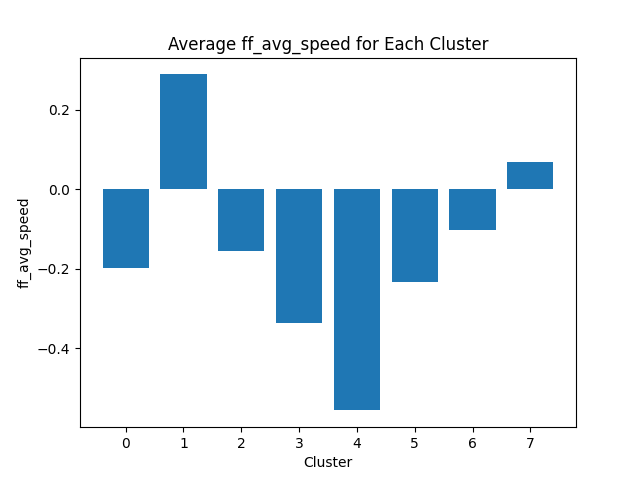
\includegraphics[scale = .5]{figs/cls_ff_vel.png}
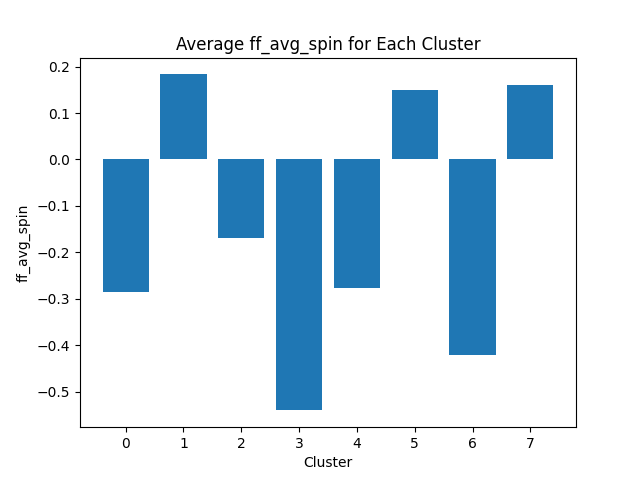
\includegraphics[scale = .5]{figs/cls_ff_spin.png}
\begin{center}Figs 10, 11: Cluster Fastball Characteristics\end{center}

Note that cluster 5 also throws very high spin fastballs, which 
is to be expected since a cutter is a fastball with a high horizontal spin rate. Clearly this 
clustering makes a lot of sense; it has sorted pitchers by the metrics of their pitches, and 
they throw those pitches with the best metrics the most frequently. Now, this clustering with 
these pitcher archetypes can next be used to determine which fatigue characteristics impact 
pitcher effectiveness for each classification. \\

TODO: Complete and include regression analysis on fatigue characteristics \\

\textbf{V. Results} \\
TODO

\textbf{VI. Discussion and Conclusion} \\
TODO

\pagebreak
\textbf{VII. References} \\
\\
\hypertarget{1}{[1]} David C. Phillips. Stopping on Nine: Evidence of Heuristic 
Managerial Decision-Making in Major League Baseball Pitcher Substitutions.
\emph{Southern Economic Journal} 84(2): 577-599, 2017.
\\
\hypertarget{2}{[2]} W. Jeffrey Grantham et al. The Impact of Fatigue on the Kinematics 
of Collegiate Baseball Pitchers. \emph{The Orthopaedic Journal of Sports Medicine}
2(6), 2014.
\\
\hypertarget{3}{[3]} David Whiteside et al. Variations in Pitching Performance During a 
Major League Baseball Game: What Can We Learn From Ball Tracking Data? 
\emph{International Conference of Biomechanics in Sports} 33, 2016
\\
\hypertarget{4}{[4]} Michael Woodham et al. When to Pull Starting Pitchers in Major League Baseball? A Data Mining Approach.
\emph{Applied Data Science}, 2016


\pagebreak
\textbf{Appendix I: Link to Data and Code} \\
\\
Full data and code may be found at: \url{https://github.com/Espeer5/PullingPitchers}

\end{document}